\chapter{Stand der Technik}

In diesem Kapitel betrachten wir zunächst, weshalb sich die Apple Watch als Smartwatch für unseren Prototypen eignet. Anschließend wird vorgestellt, wie sich deklarative User Interfaces mit SwiftUI realisieren lassen. Schließlich werden noch Bluetooth, die Persistenz von Daten und die Kommunikation zwischen iPhone und Apple Watch diskutiert.

\section{Die Apple Watch als Smartwatch}

Im September 2017 verkündete Apple, dass die Apple Watch die Nummer Eins der meistverkauften Uhren geworden ist\footnote{Ab Minute 18: \url{https://podcasts.apple.com/de/podcast/apple-special-event-september-2017/id275834665?i=1000430692674}}. Auch wir möchten die Apple Watch als Smartwatch verwenden, für die wir die App schreiben wollen. Die tiefe Integration von Watch und iPhone dient als eine gute Basis für unseren Prototypen.

\section{Deklarative User Interfaces mit SwiftUI}

Vorgestellt mit den Worten \doublequotes{Objective-C without the C}\cite{Apple::WWDC-2014}, veröffentlichte Apple 2014 eine eigene Programmiersprache: Swift \cite{Apple::Swift-Documentation}.
Swift ist eine Apple's eigener Ansatz für die Entwicklung nativer Anwendungen für iPhone und Co.

2019 folgte ein Framework zur deklarativen Programmierung nativer \aclp{UI} für iOS, watchOS und alle anderen Betriebssysteme von Apple\footnote{Ab iOS 13 und watchOS 6.}: \emph{SwiftUI} \cite{Apple::SwiftUI}. SwiftUI baut auf den bis dahin verwendeten Frameworks UIKit (iOS), WatchKit (watchOS) und AppKit (macOS) auf, die einen imperativen Ansatz verfolgen. Um den Unterschied von deklarativer und imperativer Programmierung zu verstehen, schauen wir uns ein kleines Beispiel an.

\subsection{Ein simples Beispiel}

Wir wollen eine Oberfläche mit einem Label und Eingabefeld realisieren, in das der Nutzer seinen Namen eintragen kann. Das Label soll dann eine Begrüßung mit diesem Namen anzeigen. \autoref{fig:ui:greeting} zeigt das Endergebnis.
\clearpage

\begin{figure}[H]
	\centering
	\includegraphics[width=.8\textwidth]{./images/methodology/swiftui/greeting_ui.png}
	\caption{\label{fig:ui:greeting}Einfache Oberfläche mit Label und Eingabefeld.}
\end{figure}

\subsubsection{Imperative Programmierung mit UIKit}

\begin{bsp}
Wir schauen uns zunächst an, wie wir dieses Ergebnis mithilfe imperativer Programmierung und UIKit realisieren können. Das \acl{UI} kann mit Xcode in einem Storyboard schnell realisiert werden, indem zwei \texttt{UILabel} und ein \texttt{UITextField} platziert werden. Für das obere \texttt{UILabel} wird nun ein Outlet \ref*{lst:uikit-greeting-outlet-label} und für das \texttt{UITextField} ein Outlet \ref*{lst:uikit-greeting-outlet-tf} und eine Action \ref*{lst:uikit-greeting-action-tf} in der zugehörigen \texttt{ViewController}-Klasse (\autoref{lst:uikit-greeting}) mit dem Storyboard verknüpft. Als Alternative zu Storyboards, können Oberflächen in Xcode auch mit Swift-Code aufgebaut werden. Diese Variante wollen wir hier nicht weiter verfolgen, da wir lediglich die Unterschiede zwischen imperativer und deklarativer Programmierung betrachten wollen.
	
\begin{lstlisting}[caption={\texttt{ViewController.swift}},label={lst:uikit-greeting}]
class ViewController: UIViewController {
    /*!\annotation{lst:uikit-greeting-outlet-label}!*/ @IBOutlet weak var label: UILabel!
    /*!\annotation{lst:uikit-greeting-outlet-tf}!*/ @IBOutlet weak var textField: UITextField!

    /*!\annotation{lst:uikit-greeting-action-tf}!*/ @IBAction func textFieldValueChanged(_ sender: Any) {
        guard let newText = textField.text else {
            return
        }
        label.text = "Hallo, \(newText)"
    }
}
\end{lstlisting}
\setcounter{lstannotation}{0}

Bei jeder Eingabe wird die Funktion \texttt{textFieldValueChanged(\_:)} aufgerufen. Hier wird zunächst geprüft, ob \texttt{textField.text} vom Typ \texttt{String?} ausgepackt werden kann, also nicht \texttt{nil} ist. Ist dies möglich, wird der Text des Labels neu gesetzt.

Möchte der Nutzer die Tastatur verschwinden lassen, muss dies über das \texttt{UI\-Text\-Field\-De\-le\-gate} separat implementiert werden. Bei einem Tap auf die Return-Taste passiert aktuell noch nichts.
\end{bsp}

\subsubsection{Deklarative Programmierung mit SwiftUI}

\begin{bsp}
Wie eine deklarative Programmierung mit SwiftUI \cite{Apple::SwiftUI-Documentation} aussehen kann, zeigt \autoref{lst:swiftui-greeting}. Ein \acl{UI}-Element in SwiftUI ist keine Klasse, sondern eine Struktur. Anders als Klassen, die in Swift Referenztypen sind, sind Strukturen Werttypen.

Zunächst deklarieren wir die Konformität zum \texttt{View}-Protokoll \ref*{lst:swiftui-greeting-struct}. Dieses Protokoll verlangt es, die Computed Property \texttt{body} \ref*{lst:swiftui-greeting-body} zu implementieren.

Unsere private Variable \texttt{name} \ref*{lst:swiftui-greeting-name} wird mit einem leeren \texttt{String} initialisiert. Die \texttt{@State}-Annotation ist ein sogenannter \doublequotes{Property Wrapper}. In \autoref{sec:swiftui:dependencies} wird genauer auf den Datenfluss durch SwiftUI eingegangen. Wichtig ist an dieser Stelle nur zu wissen, dass durch Manipulation einer mit \texttt{@State} annotierten Variable, die \texttt{body}-Property neu berechnet wird und dabei den geänderten Wert von \texttt{name} benutzt.

Das Keyword \texttt{some} \ref*{lst:swiftui-greeting-some} ist ein mit Swift 5.1 neu eingeführtes Feature der \doublequotes{Opaque Types}. Hier bedeutet es, dass der Rückgabe-Typ von \texttt{body} das Protokoll \texttt{View} implementieren muss. Uns ist dabei egal, von welchem Typ genau \texttt{body} ist. Es könnte sich um ein \texttt{Text}, ein \texttt{TextField} oder aber, wie hier, ein \texttt{VStack} \ref*{lst:swiftui-greeting-vstack} handeln.

Eine wichtige Sache, die man bei der Implementierung mit SwiftUI im Hinterkopf haben sollte, ist, dass für SwiftUI alles eine \texttt{View} ist und eine \texttt{View} auch nicht immer den gesamten Bildschirminhalt beschreibt. Eine \texttt{View} kann alles sein: Von der \texttt{NavigationView} mit Menüführung, über eine Liste (\texttt{List}) bis hin zum einfachen \texttt{Text}. Auch der \texttt{VStack} implementiert das \texttt{View}-Protokoll und erfüllt damit den Rückgabetyp von \texttt{some View}. Es sei angemerkt, dass das Schlüsselwort \texttt{return} in Swift optional ist, solange der Compiler erkennen kann, was zurückgegeben werden soll.

Innerhalb der geschweiften Klammern des \texttt{VStack} erwartet Swift nun weitere zu \texttt{View} konforme Elemente, die vertikal angeordnet werden sollen. Hier handelt es sich dabei um einen \texttt{Text} und einen \texttt{HStack}. Innerhalb des \texttt{String} \ref*{lst:swiftui-greeting-text} nutzen wir die \doublequotes{String-Interpolation}. Ausdrücke innerhalb der Zeichen \texttt{\textbackslash(...)} werden ausgewertet und in die Zeichenkette eingebaut.

Innerhalb des \texttt{HStack}, der Elemente horizontal anordnet, platzieren wir einen weiteren \texttt{Text} und ein \texttt{TextField} \ref*{lst:swiftui-greeting-textfield}. Der Konstruktor \texttt{init(\_:text:)} erwartet einen Platzhalter-Text und eine Variable für den Inhalt des Feldes vom generischen Typ \texttt{Binding<String>}. Der Typ \texttt{Binding<T>} wird ebenfalls genauer in \autoref{sec:swiftui:dependencies} vorgestellt. An dieser Stelle reicht es aus, das Dollar-Zeichen \$ als eine Art Referenz auf unsere private Variable \texttt{name} \ref*{lst:swiftui-greeting-name} zu sehen. Intern ist in Swift ein \texttt{String} als \texttt{struct} realisiert und damit ein Werttyp. SwiftUI löst auch das Problem der Bildschirmtastatur, indem es diese automatisch bei Antippen des Eingabefeldes anzeigt und mit Auswahl der Return-Taste verschwinden lässt.

Würden wir diesen Code ausführen, würde der \texttt{HStack} bis zum Rand des Displays ragen. Um einen Abstand um den \texttt{HStack} herum zu erreichen, rufen wir die Methode \texttt{padding(\_:)} \ref*{lst:swiftui-greeting-padding} des \texttt{HStack} auf. Diese Methode ist ein sogenannter \doublequotes{View Modifier}. Diese können auf Elemente, die das \texttt{View}-Protokoll implementieren, aufgerufen werden und verändern diese. Konkret geben \emph{View Modifier} wieder ein Element vom Typ \texttt{View} zurück. Hier ist das wieder ein \texttt{HStack}.

\begin{lstlisting}[caption={\texttt{GreetingView.swift}},label={lst:swiftui-greeting}]
struct GreetingView: /*!\annotation{lst:swiftui-greeting-struct}!*/ View {
    /*!\annotation{lst:swiftui-greeting-name}!*/ @State private var name: String = ""
    
    /*!\annotation{lst:swiftui-greeting-body}!*/ var body: /*!\annotation{lst:swiftui-greeting-some}!*/ some View {
        /*!\annotation{lst:swiftui-greeting-vstack}!*/ VStack {
            Text("Hallo, /*!\annotation{lst:swiftui-greeting-text}!*/ \(name)!")
            HStack {
                Text("Dein Name:")
                /*!\annotation{lst:swiftui-greeting-textfield}!*/ TextField("Name", text: $name)
            }
            /*!\annotation{lst:swiftui-greeting-padding}!*/ .padding()
        }
    }
}

\end{lstlisting}
\setcounter{lstannotation}{0}
	
\end{bsp}

\subsection{Vergleich zwischen imperativer und deklarativer Programmierung}

Der Ansatz der imperativen Programmierung ist es, auf Ereignisse zu reagieren und die Oberfläche dementsprechend anzupassen. Gibt der Nutzer im ersten Code-Beispiel (\autoref{lst:uikit-greeting}) einen Buchstaben ein, muss der Text des Labels manuell aktualisiert werden, indem wir den Wert des Eingabefeldes lesen und anschließend den Wert des Labels aktualisieren. Wir rufen also immer eine Funktion auf, wenn zum Beispiel auf eine Schaltfläche geklickt oder Text in ein Eingabefeld eingegeben wird.

Imperative Programmierung kann viele Probleme hervorrufen, von denen sich die meisten um den Zustand der Oberfläche drehen. Wir müssen verfolgen, in welchem Zustand sich unser Code befindet und sicherstellen, dass unsere Benutzeroberfläche diesen korrekt wiedergibt.

Angenommen, wir haben eine Oberfläche mit zwei Schaltern, die entweder \doublequotes{an} oder \doublequotes{aus} sein können. Jeder Schalter verändert eine boolesche Variable, die sich auf die Oberfläche auswirkt. Bei zwei Booleans, \texttt{a} und \texttt{b}, haben wir insgesamt vier Zustände:

\begin{table}[H]
	\centering
\begin{tabular}{rl}
	\thead{\texttt{a}} & \thead{\texttt{b}}\\
	\midrule
	\texttt{true} & \texttt{true}\\
	\texttt{true} & \texttt{false}\\
	\texttt{false} & \texttt{true}\\
	\texttt{false} & \texttt{false}\\
\end{tabular}
\caption{Vier Zustände bei zwei Booleans.}
\end{table}

Bei zwei Booleans mag dies vielleicht noch überschaubar wirken. Handelt es sich allerdings um noch mehr oder gar andere Werte, wie Strings oder Integer-Zahlen, werden die Zustände deutlich komplexer. Eine imperative Programmierung der Benutzeroberfläche bedeutet es, zu beschreiben, \textbf{wie} die Oberfläche auf Zustandsänderungen reagieren soll.

Im Gegensatz dazu, wird bei der deklarativen Programmierung beschrieben, \textbf{was} die Oberfläche leisten soll. SwiftUI erlaubt es uns, das System über alle möglichen Zustände unserer App auf einmal zu informieren.

Wir könnten zum Beispiel festlegen, dass, wenn der Benutzer eingeloggt ist, eine Begrüßungsnachricht angezeigt wird, aber wenn er ausgeloggt ist, eine Login-Schaltfläche angezeigt wird. Wir müssen keinen Code schreiben, um uns von Hand zwischen diesen beiden Zuständen zu bewegen. Stattdessen lassen wir SwiftUI zwischen den verschiedenen Benutzeroberflächen hin und her wechseln, wenn sich der Zustand ändert. Wir legen nur fest, was angezeigt werden soll, abhängig davon, ob der Benutzer an- oder abgemeldet ist. Wenn wir also den Status der Authentifizierung ändern, aktualisiert SwiftUI die Benutzeroberfläche für uns.

Das ist es, was deklarativ bedeutet: Wir modifizieren die Benutzeroberfläche nicht von Hand. Wir definieren nur Regeln, die unser System befolgen soll, und überlassen es SwiftUI, dafür zu sorgen, wie diese Regeln umgesetzt werden.

\subsection{Weitere Vorteile durch SwiftUI}

SwiftUI bringt darüberhinaus auch noch weitere Vorteile mit sich. Der Code, den wir schreiben, ist plattformunabhängig. Oben stehender Code kann ohne Veränderung $ 1:1 $ in einem watchOS-Projekt verwendet werden. \autoref{fig:ui:watch} zeigt, wie die Benutzeroberfläche des Codes aus \autoref{lst:swiftui-greeting} auf einer Apple Watch aussieht.

\begin{figure}
	\centering
	\includegraphics[width=.3\textwidth]{./images/methodology/swiftui/watch.png}
	\caption{\label{fig:ui:watch}Die Oberfläche auf der Apple Watch.}
\end{figure}

Ebenso unterstützt SwiftUI die Lokalisierung der Anwendung. Weiter oben wurde erwähnt, dass ein \texttt{Text}-Element einen \texttt{String} erwartet. Intern wandelt Swift diesen \texttt{String} in einen \texttt{LocalizedStringKey} um und übergibt diesen an die \texttt{Text}-Komponente. Initialisieren wir das \texttt{Text}-Element hingegen direkt mit einem \texttt{LocalizedStringKey}, substituiert Swift diesen durch die entsprechende Übersetzung. \autoref{lst:swiftui-greeting-loc} zeigt, wie der Swift-Code hierfür aussehen muss. \autoref{bsp:ui:en} und \autoref{bsp:ui:fr} zeigen die Oberfläche auf Englisch und Französisch mit den zugehörigen Übersetzungs-Dateien.

\begin{lstlisting}[caption={\texttt{GreetingViewLocalized.swift}},label={lst:swiftui-greeting-loc}]
struct GreetingViewLocalized: View {
    @State private var name: String = ""

    var body: some View {
        VStack {
            Text("user.greeting \(name)")
            HStack {
                Text("user.enter")
                TextField("user.name.placeholder", text: $name)
            }
            .padding()
        }
    }
}
\end{lstlisting}\setcounter{lstannotation}{0}

\begin{figure}[ht]
\begin{minipage}{0.5\textwidth}
\begin{lstlisting}[title={\texttt{Localizable.strings (English)}},label={lst:swiftui-greeting-en}]
"user.greeting %@" = "Hello, %@!";
"user.enter" = "Your name:";
"user.name.placeholder" = "Name";
\end{lstlisting}\setcounter{lstannotation}{0}
\begin{figure}[H]
\centering
\includegraphics[width=.6\textwidth]{./images/methodology/swiftui/watch-en.png}
\caption{\label{bsp:ui:en}Das englische Interface.}
\end{figure}
\end{minipage}
\begin{minipage}{0.5\textwidth}
\begin{lstlisting}[title={\texttt{Localizable.strings (French)}},label={lst:swiftui-greeting-fr},language=Swift]
"user.greeting %@" = "Salut, %@!";
"user.enter" = "Ton nom:";
"user.name.placeholder" = "Nom";
\end{lstlisting}\setcounter{lstannotation}{0}
\begin{figure}[H]
\centering
\includegraphics[width=.6\textwidth]{./images/methodology/swiftui/watch-fr.png}
\caption{\label{bsp:ui:fr}Das französische Interface.}
\end{figure}
\end{minipage}
\end{figure}

Doch hier enden die Möglichkeiten mit SwiftUI noch nicht. Zusätzlich bringt das Framework weitere Funktionalitäten, wie etwa eine Unterstützung des \emph{Dark Modes}, automatische Anpassungen der Schriftgröße nach Wünschen des Nutzers oder die Sprachausgabe für Menschen mit Sehbeeinträchtigungen durch \emph{VoiceOver}, mit sich.

\subsection{Abhängigkeiten}\label{sec:swiftui:dependencies}

Wir haben bereits den \emph{Property Wrapper} \texttt{@State} kennengelernt. Eine mit \texttt{@State} annotierte Variable ist eine \doublequotes{Source of Truth}\footnote{Dieses Wort ist sehr schnell zu einem Buzzword der WWDC 2019 geworden, auf der Apple SwiftUI vorgestellt hat.} (dt. \doublequotes{Quelle der Wahrheit}) \cite{Apple::SwiftUI-Documentation}.

\subsubsection{\doublequotes{Sources of Truth} und \doublequotes{Derived Values}}

Im Kontext der Programmierung von Benutzerschnittstellen bedeutet dies, dass wir auf redundante Speicherung von Informationen verzichten sollen. In \autoref{lst:swiftui-greeting} deklarieren wir unsere Variable \texttt{name} mit \texttt{@State} als \emph{Source of Truth}. In diesem Kontext erschließt sich die Redundanz noch nicht sofort. Wenn wir uns allerdings eine umfangreichere App vorstellen, kann es sein, dass wir an mehreren Stellen den Namen des Nutzers anzeigen oder auch verändern wollen. Würden wir in jeder einzelnen \texttt{View} eine eigene Variable \texttt{name} definieren, müssten wir auch dafür sorgen, alle Variablen aktuell zu halten. Als Werttyp kann eine \texttt{View} nämlich keine Referenzen auf lokale Variablen bereitstellen.

Eine weitere Funktion des \texttt{State} ist der, dass SwiftUI sich um die Speicherung und \doublequotes{Überwachung} aller Variablen kümmert, die als Zustand deklariert werden. Wenn sich der Wert ändert, verliert eine \texttt{View} ihre Gültigkeit und berechnet den \texttt{body} neu.

Um einen \texttt{State} an eine andere \texttt{View} in der Hierarchie zu übergeben, muss der Variablenname mit vorangestelltem \$-Zeichen verwendet werden. Dadurch wird eine Bindung auf den \texttt{State} abgerufen. In der aufgerufenen \texttt{View} wird dann die Variable nicht mit \texttt{@State} deklariert. Hier wird \texttt{@Binding} genutzt. Eine Bindung ist keine \emph{Source of Truth}, sondern ein \doublequotes{Derived Value} (dt. \doublequotes{Abgeleiteter Wert}).

Auch \texttt{@Binding} sogt für eine Aktualisierung der \texttt{View}, sobald sich der Wert des referenzierten \texttt{State}, also der \emph{Source of Truth}, ändert. Intern sorgt Swift dafür, dass alle annotierten Variablen auf die gleiche Speicherzelle auf dem Stack zeigen. In \autoref{lst:swiftui-greeting} erwartet das Eingabefeld eine Bindung auf den \texttt{State}, die wir durch das \$-Zeichen bekommen.

\subsubsection{Binden von Klassen durch \doublequotes{ObservableObjects}}

Angenommen, wir haben eine eigene Klasse, die sich um das Modell der App kümmert. \texttt{@State} können wir in der Wurzel der View-Hierarchie nicht verwenden, um eine \emph{Source of Truth} unseres Modells zu deklarieren. Hierfür nutzen wir das von SwiftUI bereitgestellte Protokoll des \texttt{ObservableObject}.

Unser Modell in \autoref{lst:swiftui-model} implementiert dieses Protokoll \ref*{lst:swiftui-model-protocol}. Hierdurch erhält die Klasse die Variable \texttt{objectWillChange}, einen \emph{Publisher}. Ein \emph{Publisher} wird dazu genutzt, Bindungen für die \texttt{Views} bereitzustellen. Sobald eine Variable des Modells verändert wird \ref*{lst:swiftui-model-willset}, muss die Funktion \texttt{send()} \ref*{lst:swiftui-model-send} unseres \emph{Publishers} \texttt{objectWillChange} aufgerufen werden. Anschließend können wir den neuen Wert (Zugriff innerhalb des \texttt{willSet}-Blocks über \texttt{newValue}) beispielsweise auf ein Server-Backend hochladen, um die Daten zu persistieren.

Anstatt für jede einzelne Variable manuell \texttt{send()} aufzurufen, stellt Swift die \texttt{@Published}-Annotation \ref*{lst:swiftui-model-published} zur Verfügung. Diese sorgt dafür, dass automatisch vor jedem Setzen der Variable, die Funktion \texttt{send()} des \emph{Publishers} aufgerufen wird.

\begin{lstlisting}[caption={Model.swift},label={lst:swiftui-model}]
final class Model: /*!\annotation{lst:swiftui-model-protocol}!*/ ObservableObject  {
    var age: Int = 0 {
        /*!\annotation{lst:swiftui-model-willset}!*/ willSet {
            /*!\annotation{lst:swiftui-model-send}!*/ objectWillChange.send()
            // Neuen Wert z. B. auf Server-Backend abspeichern.
        }
    }
    /*!\annotation{lst:swiftui-model-published}!*/ @Published var name: String = "" /* {
        willSet {
            // objectWillChange.send() wird automatisch aufgerufen.
            // Neuen Wert z. B. auf Server-Backend abspeichern.
        }
    } */
}
\end{lstlisting}\setcounter{lstannotation}{0}

Innerhalb einer \texttt{View} (\autoref{lst:swiftui-model-view}) haben wir zwei Möglichkeiten, auf die Nachrichten eines \emph{Publishers} zu reagieren. Wir können unser Modell entweder mit \texttt{@ObservedObject} \ref*{lst:swiftui-model-obs}\ref*{lst:swiftui-model-obs2} oder \texttt{@EnvironmentObject} \ref*{lst:swiftui-model-env} annotieren. Anschließend kann das Modell in der \texttt{View} verwendet werden \ref*{lst:swiftui-model-usage}. 

Im Beispiel wurden noch keine Instanzen\footnote{Es sei angemerkt, dass im Beispiel nicht dafür gesorgt wird, beide Modelle synchron zu halten. Es würden zwei Instanzen und damit zwei \emph{Sources of Truth} des Modells auf dem Stack existieren. Es sollte selbstverständlich nur eine einzige Instanz existieren.} des Modells erzeugt. Für ein \texttt{ObservedObject} muss dieses entweder in der \texttt{ModelView} initialisiert \ref*{lst:swiftui-model-obs2} oder beim Aufruf des Konstruktors der \texttt{ModelView} übergeben werden \ref*{lst:swiftui-model-obs}. Dies geschieht in der aufrufenden \texttt{ParentView} über \texttt{ModelView(model: Model())}. Möchte unsere \texttt{ModelView} das Objekt an eine untergeordnete \texttt{View} übergeben, geschieht das ebenfalls über den Konstruktor \texttt{SubView(model: modelObs)} \ref*{lst:swiftui-model-sub}. Alternativ kann auch direkt ein Bindung mit beispielsweise \texttt{\$modelObs.name} an die untergeordnete \texttt{View} übergeben werden

 Bei der Übergabe eines Modells an andere \texttt{Views} kann es bei einer großen \texttt{View}-Hierarchie schnell unübersichtlich werden. Abhilfe schafft \texttt{@EnvironmentObject} \ref*{lst:swiftui-model-env}. Hierzu wird die Instanz des Modells an eine Wurzel-\texttt{View} mit  \texttt{RootView().environmentObject(Model())} übergeben. Dies passiert bei einem neuen Xcode-Projekt üblicherweise im \texttt{SceneDelegate}. Alle dieser Wurzel untergeordneten \texttt{Views} können nun mit \texttt{@EnvironmentObject} auf diese Instanz automatisch zugreifen. Swift kümmert sich darum, das Modell zur Verfügung zu stellen und einzubinden.

\begin{lstlisting}[caption={ModelView.swift},label={lst:swiftui-model-view}]
struct ModelView: View {
    /*!\annotation{lst:swiftui-model-obs}!*/ @ObservedObject var modelObs: Model
    // Oder bei Initialisierung innerhalb der View:
    // /*!\annotation{lst:swiftui-model-obs2}!*/ @ObservedObject var modelObs: Model = Model()
    /*!\annotation{lst:swiftui-model-env}!*/ @EnvironmentObject var modelEnv: Model
    
    var body: some View {
        VStack {
            /*!\annotation{lst:swiftui-model-usage}!*/ Text("\(modelObs.name) ist \(modelEnv.age) Jahre alt.")
            /*!\annotation{lst:swiftui-model-sub}!*/ SubView(model: modelObs)
        }
    }
}
\end{lstlisting}\setcounter{lstannotation}{0}

Es gibt keine Regel, wann ein \texttt{State}, ein \texttt{ObservedObject} oder ein \texttt{EnvironmentObject} zu verwenden sind. Dies kann nur für den jeweiligen Einsatzzweck entschieden werden. \texttt{States} sind dann zu empfehlen, wenn die jeweilige \texttt{View} alleinigen Zugriff benötigt. Bei multiplen Zugriffen sollte ein \texttt{ObservableObject} verwendet werden, abhängig davon, wie groß die \texttt{View}-Hierarchie ist und an welchen Stellen die Daten benötigt werden. \autoref{tab:data-flow} zeigt noch einmal alle möglichen Wege des Datenflusses mit SwiftUI auf.

\begin{table}[H]
\centering
\begin{tabular}{c|cc}
& \emph{Source of Truth} & \emph{Derived Value}\\
\hline&&\\
Read-only & Konstante & Property\\&&\\
Read-write & \makecell{\texttt{@State}\\\texttt{ObservableObject}} & \makecell{\texttt{@Binding}\\\texttt{@ObservedObject}\\\texttt{@EnvironmentObject}}\\
\end{tabular}
\caption{\label{tab:data-flow}Übersicht über die verschiedenen Datenfluss-Arten in SwiftUI.}
\end{table}

\section{Bluetooth Low Energy mit CoreBluetooth}\label{sec:bluetooth}

Für die drahtlose Kommunikation mit  Bluetooth existieren mehrere Arten. Die bekanntesten sind \doublequotes{Bluetooth Classic}, \doublequotes{\acl{BLE}} und \doublequotes{iBeacon}.

\subsection{Bluetooth Classic, Bluetooth Low Energy und iBeacon}

\acl{BT Classic} und \acl{BLE} sind von der \doublequotes{Bluetooth Special Interest Group} herausgegebene Standards zur drahtlosen Kommunikation zwischen Geräten \cite{Group:2019:Bluetooth-Core-Specification}. Der ursprüngliche Standard, \ac{BT Classic}, der früher nur \doublequotes{Bluetooth} genannt wurde, kann beispielsweise genutzt werden, um Dateien zwischen Geräten zu übertragen oder drahtlose Kopfhörer mit einem Gerät zu verbinden. Ein großer Nachteil von \ac{BT Classic} ist allerdings der hohe Stromverbrauch. Gerade für Geräte, die nur gelegentlich Daten kleiner Größe austauschen, braucht es keine permanente Verbindung, die in der Lage ist, Audiosignale zu übertragen. 

Mit \ac{BLE} existiert ein weiterer Standard, der -- wie der Name schon sagt -- sehr stromsparend ist. Er wurde mit der \emph{Bluetooth Core Specification 4.0} eingeführt. Der Standard basiert auf einer Client-Server-Architektur. Clients werden als \doublequotes{Centrals} bezeichnet. \emph{Centrals} versuchen, auf die Daten der Peripheriegeräte (\emph{Peripherals}), den Servern, zuzugreifen. Peripheriegeräte stellen die Eigenschaften (\emph{Characteristics}) durch Werte dar. Zusammengehörige Eigenschaften werden in einem übergeordneten Konstrukt zusammengefasst, das als \emph{Service} bezeichnet wird. Eine Eigenschaft besitzt keinen oder mehrere Deskriptoren (\emph{Descriptors}). Diese können verschiedene Arten von Metadaten enthalten, mit denen sie die verknüpfte Charakteristik ergänzen können. Mithilfe des \ac{CCCD} können beispielsweise die Benachrichtigungen durch die Peripheriegeräte empfangen werden. \autoref{dia:ble} veranschaulicht den Zusammenhang der einzelnen Komponenten.

Jeder \emph{Service}, jede \emph{Charakteristic} und jeder \emph{Descriptor} muss durch einen eindeutigen Bezeichner, einen \ac{UUID}, identifiziert werden können. \acp{UUID} können 16- oder 128-Bit-Werte sein und zum Beispiel mit \texttt{uuidgen} in einer Bash generiert werden.

Zudem ist es möglich, \ac{BLE}-Geräte ad-hoc miteinander zu verbinden, ohne vorher eine explizite Verbindung (\emph{Pairing}) zu initiieren. Ein explizites \emph{Pairing} ist nur für verschlüsselte Übertragungen notwendig.

\begin{figure}[ht]
	\begin{adjustbox}{scale=0.7,center} % 	\begin{adjustbox}{scale=0.7,center}
		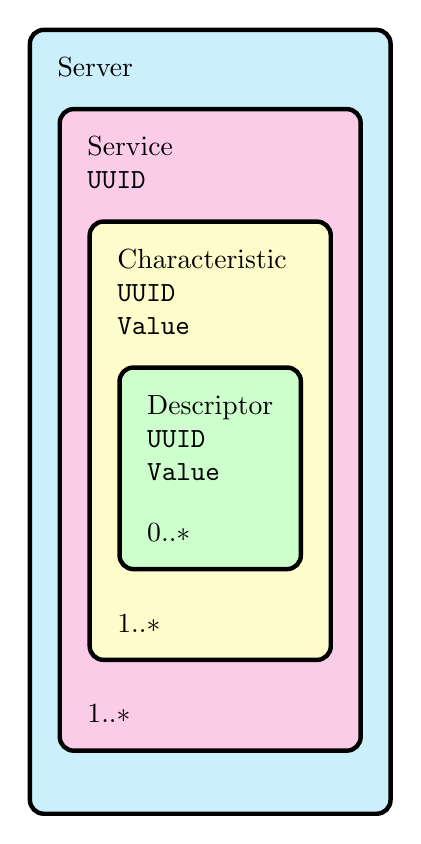
\begin{tikzpicture}
		\tikzstyle{all} = [draw, ultra thick, align=left]
		\tikzstyle{block} = [rectangle, all, inner sep=1em, rounded corners=5pt]
		\node[block, fill=cyan!20] {
			Server\\[1em]
			\tikz \node[block, fill=magenta!20] {
				Service\\{\ttfamily UUID}\\[1em]
				\tikz \node[block, fill=yellow!20] {
					Characteristic\\{\ttfamily UUID}\\{\ttfamily Value}\\[1em]
					\tikz \node[block, fill=green!20] {
						Descriptor\\{\ttfamily UUID}\\{\ttfamily Value}\\[1em]$0..*$
					};\\[1em]$1..*$
				};\\[1em]$1..*$
			};\\
		};
		\end{tikzpicture}
	\end{adjustbox}
	\caption{\label{dia:ble}Aufbau eines BLE-Peripheriegeräts. Nach \cite{Kolban:2018:BLE-C-Guide}}
\end{figure}

iBeacon ist ein von Apple eingeführter Standard, der auf \ac{BLE} aufbaut, der zur Lokalisierung von Geräten genutzt wird \cite{Apple-Inc.::iBeacon}\cite{Hiramatsu:2017:Outdoor-Studying-System}. Ein iBeacon kann keine Daten empfangen, speichern oder Benachrichtigungen senden. Gesendet werden nur die eigene \ac{UUID}, sowie die Werte \emph{Major} und \emph{Minor}, beide vorzeichenlose Integer zwischen 0 und 65535.

\subsection{Core Bluetooth}

Für die Bluetooth-Kommunikation stellt Apple das \doublequotes{\acl{CB}}-Framework (\acs{CB}) bereit \cite{Apple-Inc.::Core-Bluetooth}. Dieses Framework bietet Unterstützung für \ac{BT Classic} und \ac{BLE}. iBeacon ist Bestandteil des \doublequotes{Core Location}-Frameworks, da es von Apple nur für die Positionsbestimmung vorgesehen ist. Die iBeacon-Technologie wird in dieser Arbeit nicht weiter verfolgt.

Das \ac{CB}-Framework unterstützt für \ac{BLE} grundsätzlich beide Betriebsmodi\footnote{Der Xcode Simulator unterstützt seit iOS 7 kein \acl{CB} mehr. Zum Testen, wird ein physisches Gerät benötigt.}. Ein iOS-Gerät kann sowohl als Client (\emph{Central}), als auch als Server (\emph{Peripheral}) agieren und Verbindungen auch im Hintergrund nutzen. Bei einer Implementierung ist es wichtig zu wissen, dass iOS-Geräte, die im Hintergrund einen \emph{Service} bereitstellen, nur von anderen iOS-Geräten gefunden werden können und auch nur, wenn diese explizit nach den \emph{Service}-\acp{UUID} suchen\footnote{\url{https://developer.apple.com/library/archive/documentation/NetworkingInternetWeb/Conceptual/CoreBluetooth_concepts/CoreBluetoothBackgroundProcessingForIOSApps/PerformingTasksWhileYourAppIsInTheBackground.html\#//apple_ref/doc/uid/TP40013257-CH7-SW9}}!

Bei der Apple Watch sind die Funktionalitäten deutlich eingeschränkter. Mit Bluetooth als wichtigste Kommunikationsschnittstelle, steht \acl{CB} unter watchOS nur eingeschränkt zur Verfügung, um sicherzustellen, dass alle Systemaktivitäten ausgeführt werden können. Die Apple Watch kann nur als \emph{Central} agieren und höchstens zwei Peripheriegeräte gleichzeitig verwenden. Verbindungen zu \emph{Peripherals} werden zudem getrennt, sobald die App angehalten wird.

\section{Speicherung von Daten in der iCloud}

Mit der iCloud hat Apple eine einfache Möglichkeit geschaffen, Cloud-Backups von Geräten zu erstellen und Dateien beziehungsweise Daten zwischen verschiedenen Geräten zu synchronisieren. Es gibt drei Arten, die iCloud in einer App zu verwenden: als Schlüssel-Wert-Paare (\emph{Key-Value}-Speicher), in einer Art Datenbank (\emph{CloudKit}) oder auf Dateiebene (\emph{iCloud Drive}).

Wir wollen hier nur die erste Variante betrachten. \emph{CloudKit} ist für eine kleine Anwendung, wie wir sie schreiben, viel zu mächtig. Einen datenbankähnlichen Speicher benötigen wir für die Speicherung einzelner Attribute nicht. Da \emph{iCloud Drive} hauptsächlich für dokumentenbasierte Anwendungen, wie etwa Apples eigene Office-Lösungen \emph{Pages}, \emph{Numbers} und \emph{Keynote}, interessant ist, wollen wir uns nur der ersten Variante widmen.

\subsection{Key-Value Speicher}

Diese Art der Synchronisation ist dazu gedacht, kleine Daten zwischen den Geräten auszutauschen. Maximal können im \emph{Key-Value}-Speicher der iCloud 1024 Einträge gespeichert werden, der insgesamt nicht größer als \SI{1}{\mega\byte} sein darf. Die Länge eines Schlüssels ist auf  \SI{64}{\byte} begrenzt \cite{Kofler:2019:Swift-5---Das-umfassende-Handbuch}. Leider unterstützt watchOS diese iCloud-Variante nicht. \autoref{sec:user-defaults} zeigt, wie Daten lokal auf der Apple Watch gespeichert werden können und in \autoref{sec:watch-connectivity} wird die Kommunikation zwischen iPhone und Apple Watch vorgestellt.

Die Klasse \texttt{NSUbiquitousKeyValueStore} ist Bestandteil des \texttt{Foundation}-Frameworks, welches die grundlegendste Bibliothek von Swift ist. Nach Aktivierung \emph{Key-Value-Capability} in Xcode und Erzeugen der Instanz \ref*{lst:cloud-init} in \autoref{lst:cloud-kv}, kann der Speicher ganz leicht verwendet werden.

Um einen Wert zu speichern, wird die Methode \texttt{set(\_:forKey:)} \ref*{lst:cloud-set} genutzt. Diese ist mehrfach vorhanden und akzeptiert viele Datentypen, wie etwa \texttt{String}, \texttt{Data} oder auch \texttt{Any}.

Gelesen wird ein Wert mit Aufruf der Methode, die dem erwarteten Typ entspricht. Um einen \texttt{String} zu lesen, wird die Methode \texttt{string(forKey:)} \ref*{lst:cloud-get} verwendet. Die Methode \texttt{object(forKey:)} gibt uns beispielsweise ein Objekt vom Typ \texttt{Any?} zurück. Viele Methoden, die zum Lesen von Werten gedacht sind, geben uns ein \texttt{Optional} dieses Typs wieder, da nicht für jeden Schlüssel ein Wert ermittelt werden kann.

\begin{lstlisting}[caption={Storage.swift},label={lst:cloud-kv}]
final class Storage {
    /*!\annotation{lst:cloud-init}!*/ static let kvStore = NSUbiquitousKeyValueStore()
    
    func setString(key: String, value: String) {
        /*!\annotation{lst:cloud-set}!*/ kvStore.set(value, forKey: key)
    }
    
    func getString(key: String) -> String? {
        /*!\annotation{lst:cloud-get}!*/ kvStore.string(forKey: key)
    }
}
\end{lstlisting}\setcounter{lstannotation}{0}

Bei Verwendung dieses Speichers, behält das Gerät eine lokale Kopie der Daten. Nicht immer ist eine Verbindung mit dem Internet und damit der iCloud vorhanden. Um die Synchronisation der beiden Kopien kümmert sich das Betriebssystem. Ein Aufruf der \texttt{synchronize()}-Methode erzwingt dies, wenn es möglich ist.

\subsection{Lokale Alternative mit User-Defaults}\label{sec:user-defaults}

Um Schlüssel-Wert-Paare nur lokal zu speichern eignen sich auch die \emph{User-Defaults}. Falls keine geräteübergreifende Synchronisation gewünscht ist, können statt des \texttt{NS\-Ubiq\-ui\-tous\-Key\-Value\-Store} die \emph{User-Defaults} verwendet werden. Ersetzt man in \autoref{lst:cloud-kv} \doublequotes{\texttt{NS\-Ubiq\-ui\-tous\-Key\-Value\-Store()}} \ref*{lst:cloud-init} durch \doublequotes{\texttt{UserDefaults.standard}}, hat man eine Lösung, die Daten lokal persistiert. Diese Variante steht unter watchOS zur Verfügung.

\section{Kommunikation zwischen iPhone und Apple Watch}\label{sec:watch-connectivity}

Für die Kommunikation zwischen iPhone und Apple Watch existiert das \emph{WatchConnectivity}-Framework. Nach Herstellen der Session beim Start der Apps, können Nachrichten auf mehrere Arten gesendet werden. Neben dem Transfer von Dateien und Information für \emph{Komplikationen} des \emph{Watchfaces}, gibt es drei Methoden, die einfache Nachrichten verschicken. Diese akzeptieren jeweils ein \emph{Dictionary} vom Typ \texttt{[String: Any]}.

Die einfachste Art wird mit \texttt{WC\-Session.default.send\-Message(\_:reply\-Handler:error\-Handler:)} verschickt. Diese Methode verschickt die Nachricht nur, wenn die App auf beiden Geräten im Vordergrund läuft. Dann ist der \texttt{activation\-State} der Session gleich \texttt{WC\-Session\-Activation\-State.activated}. Wurde die Nachricht übertragen, wird der \texttt{reply\-Handler} aufgerufen, bei Fehlern der \texttt{error\-Handler}.

Möchte man Nachrichten an die geschlossene \emph{Counterpart}-App übertragen, kann man die Methoden \texttt{updateApplicationContext(\_:)} und \texttt{transfer\-User\-Info(\_:)} der Session verwenden. Beide senden das \emph{Dictionary} an das andere Gerät, das die Nachricht zwischenspeichert. Sobald die Anwendung auf diesem Gerät geöffnet wird, wird die Nachricht ausgeliefert. Der Unterschied zwischen einem \emph{Application\-Context} und einer \emph{User\-Info} ist folgender: Existiert auf dem anderen Gerät bereits ein nicht-ausgelieferter \emph{Application\-Context}, wird bei Empfang eines weiteren Kontexts der Wartende überschrieben. Auf diese Weise kann zum Beispiel ein Zustand der App übertragen werden, wenn wir nur an der letzten Version interessiert sind. Bei einem Chat wollen wir beispielsweise allerdings, dass das andere Gerät alle empfangenen Chat-Mitteilungen bekommt. Hierzu eignet sich die \emph{User\-Info}: Alle empfangenen \emph{User\-Infos} werden in einer FIFO-Queue gespeichert und bei Öffnen der App in Empfangsreihenfolge übergeben. So geht keine Nachricht verloren.
